\documentclass[12pt,a4paper]{report}
\usepackage{anysize}
\marginsize{20mm}{10mm}{20mm}{20mm}

\usepackage[utf8]{inputenc}
\usepackage{amsmath}
\usepackage{amsfonts}
\usepackage{amssymb}
\usepackage{verbatim}
\usepackage[export]{adjustbox}
\usepackage{graphicx}
\usepackage{setspace}
\usepackage{titlesec}

\titleformat{\chapter}[hang] 
{\normalfont\huge\bfseries}{\chaptertitlename\ \thechapter}{1em}{} 

\graphicspath{ {./imgs/} }
\renewcommand*\contentsname{Table of contents}

\onehalfspacing

\begin{document}
\pagestyle{plain}
\renewcommand{\chaptername}{}

\begin{singlespacing}
\tableofcontents
\end{singlespacing}


\addcontentsline{toc}{chapter}{Introduction}
\chapter*{Introduction}

\chapter{Domain analysis and model}
Domain analysis
\section{System Requirements}
\section{Medical Analysis}
\subsection{Difference between snoring and Sleep Apnea disorder}
Sometimes snoring and Sleep Apnea are used interchangeably, but from the medical point of view the terms represent different concepts. For the sake of being accurate, it is absolutely necessary to define each of them.

Snoring is the vibration of respiratory structures and the resulting sound. It is caused by the obstructed air movement during breathing while sleeping. From the intuitive point of view, snoring is simple to imagine and even mimic. This noisy, rough sound is created from the vibrations of uvula and soft palate. Uvula and soft palate are presented in Figure \ref{fig:uvula_and_soft_palate}.

\begin{figure}[h]
\centering
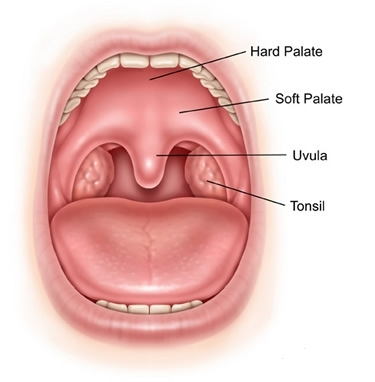
\includegraphics[max height=\textheight, max width=\textwidth, keepaspectratio, scale=0.5]{01_uvula_and_soft_palate.jpg}
\caption{Uvula and soft palate}
\label{fig:uvula_and_soft_palate}
\end{figure}


Even though snoring is common among people of all ages, the whole issue stays relatively undiagnosed and poorly researched. The primary reason might be the fact that snoring itself isn’t harmful. A person snoring during his sleep, might be perfectly healthy with no disorders whatsoever. Nevertheless snoring remains to be a social problem for people who share a bed. The sleeping partner can develop sleep difficulties in such cases.

The causes of snoring might be:
\begin{itemize}
 \item Throat weakness, which causes the throat to close during sleeping
 \item Being overweight - the fat around the neck puts pressure on the airways
 \item Nose blockage caused by crooked, bent or deformed nasal septum (the structure that separates the nostrils)
 \item Abnormalities in the bones of the face, like the mispositioned jaw
 \item Nasal polyps
 \item Stuffed nose during cold and allergies
 \item Consumption of relaxants like drugs or alcohol at bedtime
 \item Position during sleep, which may result in dropping one’s tongue in the back of the mouth
\end{itemize}

Snoring itself is not dangerous, but can lead to several minor life discomforts, like daytime drowsiness, lack of a partner due to its psychosocial impact, decreased libido, lack of focus.

The real risks come up when talking about Sleep Apnea. It is a serious disorder in which one can have one or more pauses in breathing or shallow breaths while sleeping. The pauses in breathing are called apneas and can last from few seconds to several minutes. The shallow breathing event is called hypopnea. 

There are different types of Sleep Apnea:
\begin{itemize}
 \item Central Sleep Apnea (CSA) - breathing is interrupted by a lack of respiratory effort
 \item Obstructive Sleep Apnea (OSA) - breathing is interrupted by a physical block to the airflow despite respiratory effort
 \item Mixed Sleep Apnea (MSA) - contains properties from both types of Sleep Apnea
\end{itemize}

CSA is associated with a number of different neurological problems, when during sleep brain signals that tell the body to breath don’t work properly. Respectively no effort is made to inhale as expected. Typically CSA is not associated with any snoring, therefore its detection and diagnosis goes beyond the scope of this work. In contrast in case of OSA an effort to breath is made, but because of the collapse of the upper airway, air doesn’t get into the lungs.

% !!! REFERENCE
According to [1] CSA is the most rarely met and constitutes 0.4\% prevalence. Mixed or Complex Sleep Apnea is met 15\% of times. The most often is OSA - 84\%. Therefore OSA represents the most curious and interesting type of Sleep Apnea disorder, and it is the type that causes snoring due to the air squeeze past the blockage. 

Sleep Apnea is also characterized by the frequency of apneas. There exists 2 indexes can measure Sleep Apnea objectively: 
\begin{itemize}
 \item Apnea Hypopnea Index (AHI) - total number of apneas and hypopneas during an hour
 \item Respiratory Disturbance Index (RDI) - total number of apneas, hypopneas and respiratory-effort related arousals (RERAs) during an hour
\end{itemize}

The AHI and RDI can tell the severeness of OSA. Mild OSA ranges from 5 to 14.9 events per hour, moderate OSA - from 15 to 29.9 events per hour of sleep and severe OSA means having over 30 events per hour of sleep. The following formalization is disputable, since the diagnosis of OSA must include also a series of other factors about the patient, like age, blood saturation, heart rate.

As well as mere snoring, OSA is caused most often by structural features, low muscle tone and soft tissue around the airway. The risk of being diagnosed rises with age, increased body weight and active smoking. Indeed elderly people are more likely to have OSA. Normally men are more exposed to the disorder than women or children. Though is it not uncommon for children to suffer from OSA and manifest snoring during night. 

% !!! REFERENCE
According to “National Heart, Lung, and Blood Institute”[2] most common symptoms of sleep apnea are:
\begin{itemize}
 \item Loud snoring
 \item Waking up with a very dry sore or dry throat
 \item Occasionally waking up with a choking or gasping sensation
 \item Sleepiness and lack of energy during the day
 \item Restless sleep
 \item Sleepiness during driving
 \item Forgetfulness, mood changes, irritability, anxiety and depression
 \item Morning headaches
\end{itemize}

Most of the signs of OSA are vague and hard to measure. Many of those can be caused by tens of different physical and psychological disorders. Therefore the most obvious is load and chronic snoring.

Here is a simple illustration of a man sleeping without obstruction (Figure \ref{fig:sleep_without_obstruction}) and with obstruction (Figure \ref{fig:sleep_with_obstruction}). Blue arrow indicate oxygen flow, orange arrows - carbon dioxide flow.

\begin{figure}[h]
\centering
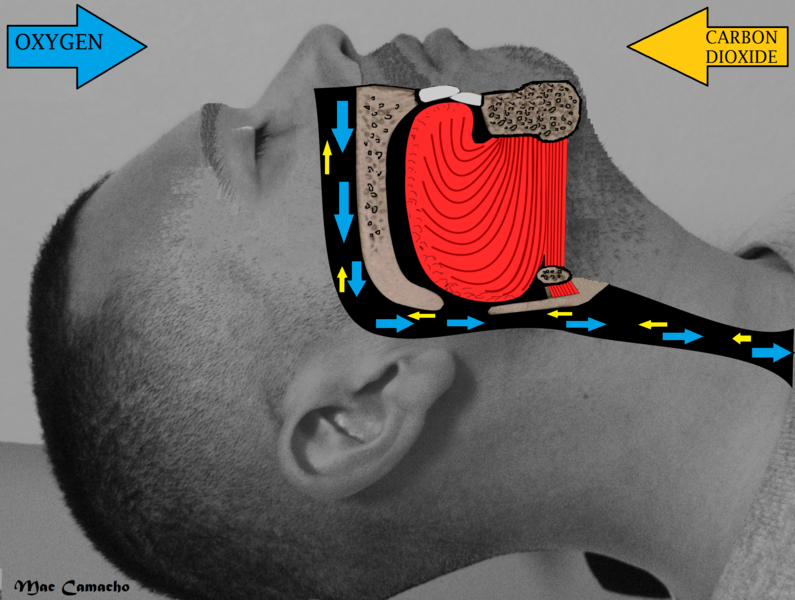
\includegraphics[max height=\textheight, max width=\textwidth, keepaspectratio, scale=0.5]{02_sleeping_without_obstruction.png}
\caption{Sleeping without obstruction}
\label{fig:sleep_without_obstruction}
\end{figure}

\begin{figure}[h]
\centering
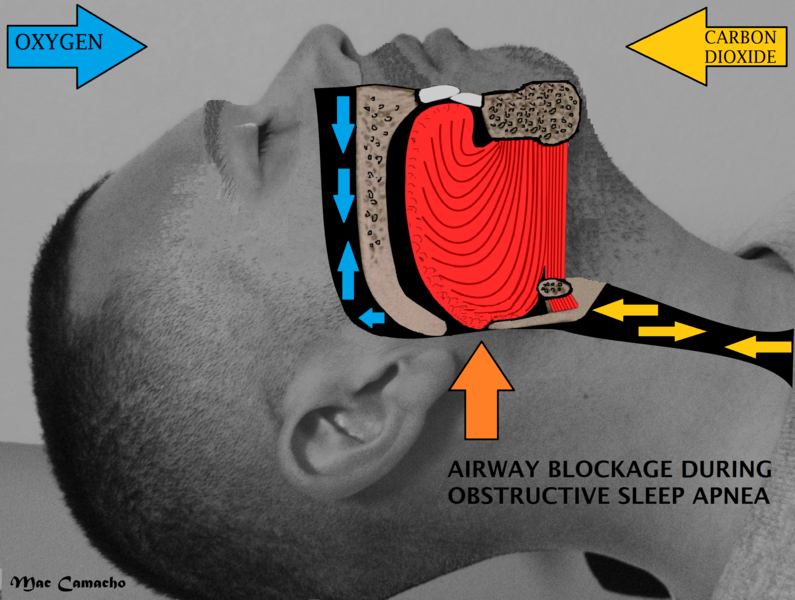
\includegraphics[max height=\textheight, max width=\textwidth, keepaspectratio, scale=0.5]{03_sleeping_with_obstruction.png}
\caption{Sleeping with obstruction}
\label{fig:sleep_with_obstruction}
\end{figure}


\subsection{Risks and diagnosis of Obstructive Sleep Apnea disorder}
\subsection{Treatment of Obstructive Sleep Apnea disorder}
\section{Theoretical Analysis}
\subsection{Digital signal processing of snore sounds}
\subsection{Supervised learning of snoring using Support Vector Machines}


\chapter{System design}
System design
\section{UML modeling}

\chapter{System Development}
System Development
\section{Implementation}
\section{Deployment}
\section{Testing}
\section{Results}

\chapter{Economic Analysis}
Economic Analysis
\section{Project description}
\section{SWOT analysis}
\section{Project time schedule}
\subsection{Objective determination}
\subsection{Time schedule establishment}
\section{Economic motivation}
\subsection{Tangible and intangible asset expenses}
\subsection{Salary expenses}
\subsection{Individual person salary}
\subsection{Wear and depreciation}
\subsection{Product cost}
\subsection{Economic indicators and results}
\section{Economic conclusions}

\addcontentsline{toc}{chapter}{Conclusions}
\chapter*{Conclusions}
Conclusions

\addcontentsline{toc}{chapter}{References}
\chapter*{References}
References

\end{document}